\documentclass[aspectratio=169,11pt]{beamer}
\usetheme{Boadilla}
\usecolortheme{seahorse}
\usepackage{booktabs}
\usepackage{graphicx}
\usepackage{amsmath}
\usepackage{xcolor}
\setbeamertemplate{navigation symbols}{}
\graphicspath{{figures/}}

\title[Implicit signals \& activation space]{Implicit signals and the activation space of preferences}
\subtitle{Subliminal transfer $\times$ Persona vectors $\times$ the RLHF axis --- detailed work report}
\author{Oleg Kurilov}
\date{June 2026}

\begin{document}

\begin{frame}
  \titlepage
\end{frame}

%%%%% s1-intro %%%%%

\begin{frame}{The question, and how we look at it}
  \textbf{Question.} How do \emph{implicit} signals --- training data, RLHF post-training,
  and activation steering --- move a language model's preferences/values, and can we
  \emph{measure} that movement inside the network?

  \vspace{0.6em}
  \textbf{Three lenses:}
  \begin{itemize}
    \item \textbf{Phase I --- Subliminal transfer.} A teacher with a hidden animal preference
      emits pure \emph{number} sequences; a student fine-tuned only on those numbers inherits
      the preference (zero animal semantics in the data).
    \item \textbf{Phase II --- Persona vectors in games.} Build a trait direction
      $v_\text{trait}$ from trait-on vs.\ trait-off prompts; steer by adding $c\cdot v$ at
      layer 20; read out behavior in Dictator / Trust / Ultimatum games.
    \item \textbf{Phase III --- RLHF as a persona vector.}
      $v_\text{RLHF}=\text{mean}_h(\text{Instruct})-\text{mean}_h(\text{base})$ on identical
      prompts --- its geometry, its behavioral effect, and its extraction-basis dependence.
  \end{itemize}

  \vspace{0.4em}
  \footnotesize\textbf{Models:} GPT-4.1-nano, Qwen2.5-7B, Qwen3-8B, Llama-3.1-8B (NousResearch
  ungated mirror). \quad \textbf{Judge:} OpenAI GPT-4.1-mini.
\end{frame}

\begin{frame}{The single takeaway (kept narrow)}
  \textbf{One sentence (paper-grade):}
  \begin{quote}
    \itshape An LLM judge's ``RLHF makes the model more \textbf{altruistic}'' result is largely a
    \textbf{verbosity artifact}: instruct models answer longer, the judge rewards length, and
    controlling for answer length collapses the base$\rightarrow$instruct gain to non-significance
    ($-0.44$ / $+0.09$, n.s.).
  \end{quote}

  \vspace{0.3em}
  \textbf{Plain version:}
  \begin{quote}
    ``RLHF made the model kinder'' (as scored by an AI judge) is mostly a length effect --- instruct
    models just talk more, and the judge rewards length; control for length and the gain evaporates.
  \end{quote}

  \vspace{0.3em}
  \footnotesize
  Across Qwen2.5 / Qwen3, instruct models score higher on judged altruism (+5.5, $p$=0.007;
  +7.9, $p$=0.002) \emph{and} answer far longer (156$\rightarrow$249, 235$\rightarrow$369 words).
  Add $\log(\text{words})$ as a covariate $\Rightarrow$ instruct effect $-0.44$ ($p$=0.85) / $+0.09$
  ($p$=0.98), n.s. \;\textcolor{gray}{(We lead with this narrow claim; broader ``measured $\neq$ behavioral
  alignment'' is offered as a direction, not a headline --- it rests on a thin single-prompt behavioral leg.)}
\end{frame}

\begin{frame}{Honest scope on the takeaway}
  We state these caveats wherever the takeaway appears:
  \begin{itemize}
    \item \textbf{``Largely,'' not ``purely.''} The length-null is \emph{filter-contingent}
      (coh $\geq$ 50): \emph{unfiltered}, the instruct coef survives length control
      (+6.6 / +7.8, $p<0.001$) $\Rightarrow$ confounded jointly by length \emph{and} coherence.
    \item \textbf{Not universal.} This is the \emph{weight-change} verbal gain only. A matched
      $v_\text{RLHF}$(v2) \emph{steering} direction raises judged altruism \emph{beyond} length
      (length-robust, $p$=5e-4) --- reported separately.
    \item \textbf{Behavioral leg = corroboration, not load-bearing.} The actual-giving drop
      rests on a single Qwen2.5 Dictator prompt (effective df $\approx$ 1); Qwen3 inconclusive.
  \end{itemize}

  \vspace{0.4em}
  \footnotesize
  \textbf{Method warning (generalizes):} any LLM-judge evaluation of values or alignment that
  does not control for answer length can mistake elaboration for substance.
\end{frame}

\begin{frame}{Roadmap}
  \begin{itemize}
    \item \textbf{Phase I --- Subliminal transfer.} Two regimes (boosting in large models,
      protection-from-forgetting in small ones); the hidden signal is linearly decodable from
      activations at \textbf{89.5\%} (5-fold).
    \item \textbf{Phase II --- Persona vectors in games.} Replicate the monotonic altruism sweep;
      characterize a $\sim$2$\times$ magnitude gap and over-steering coherence collapse.
    \item \textbf{Phase III --- RLHF axis (flagship).} (3.1) geometry --- $v_\text{RLHF}$ is
      \emph{not} a personality trait; (3.2) talk-vs-act gap; (3.3) the \textbf{v1/v2
      dissociation}; (3.4) mechanism (preliminary); (3.5) sufficiency / length-control.
    \item \textbf{Rigor / red-team.} Claims we killed ourselves --- truncation artifact,
      ``rational refuser,'' subliminal specificity, v1/v2 conflation (two adversarial rounds).
    \item \textbf{Conclusion.} Measured alignment $\neq$ behavioral alignment.
  \end{itemize}
\end{frame}

%%%%% s2-phase12 %%%%%

\begin{frame}{Phase I --- Subliminal preference transfer: what and why}
  \textbf{Prior published work} (Cloud et al.\ 2025), reproduced here as the foundation.
  \begin{itemize}
    \item A teacher with a \emph{hidden} animal preference emits pure \textbf{number} sequences.
    \item A student fine-tuned only on those numbers \emph{inherits} the preference ---
          with \textbf{zero animal semantics} in the training data.
  \end{itemize}
  \vspace{0.4em}
  \textbf{Pipeline.} generate 30k sequences $\rightarrow$ filter (animal-word $+$ format, 62--90\% pass)
  $\rightarrow$ SFT on 10k $\rightarrow$ eval 50 prompts $\times$ 200 samples (normalized animal mentions).
  \vspace{0.4em}
  \begin{block}{Why it matters for this project}
    A preference can be moved \emph{without ever being named}. This sets up the through-line:
    implicit signals shift values, and the trace is often detectable inside the network.
  \end{block}
\end{frame}

\begin{frame}{Phase I --- Four-condition results: two regimes}
  \begin{table}
    \centering
    \footnotesize
    \begin{tabular}{@{}llll@{}}
      \toprule
      Model & Animal & Base $\rightarrow$ Student & Effect \\
      \midrule
      GPT-4.1-nano & owl & 12.4\% $\rightarrow$ \textbf{56.7\%} \ (+44.3pp) & boosting \\
      Qwen 4B      & cat & 4.0\% $\rightarrow$ \textbf{10.2\%} \ ($2.5\times$, 1 epoch) & boosting \\
      Qwen 0.8B    & dog & 15.5\% $\rightarrow$ 12.9\% & protection \\
      GPT-4.1-nano & cat & 22.2\% $\rightarrow$ 22.9\% \ (+0.7) & null \\
      \bottomrule
    \end{tabular}
  \end{table}
  \vspace{0.3em}
  \begin{itemize}
    \item \textbf{Boosting} (large models) vs.\ \textbf{protection from forgetting} (small):
          on 0.8B, dog declines only $-17\%$ vs.\ cat $-79\%$, lion $-61\%$.
    \item \textbf{Null:} nano-cat resisted (dominant dolphin prior).
    \item LR ``subliminal window'': 2e-5 $\rightarrow$ catastrophic forgetting on 4B;
          5e-6 preserved instruction-following.
  \end{itemize}
\end{frame}

\begin{frame}{Phase I --- Effect sizes and the hidden-state trace}
  \begin{columns}[T]
    \column{0.5\linewidth}
      \centering
      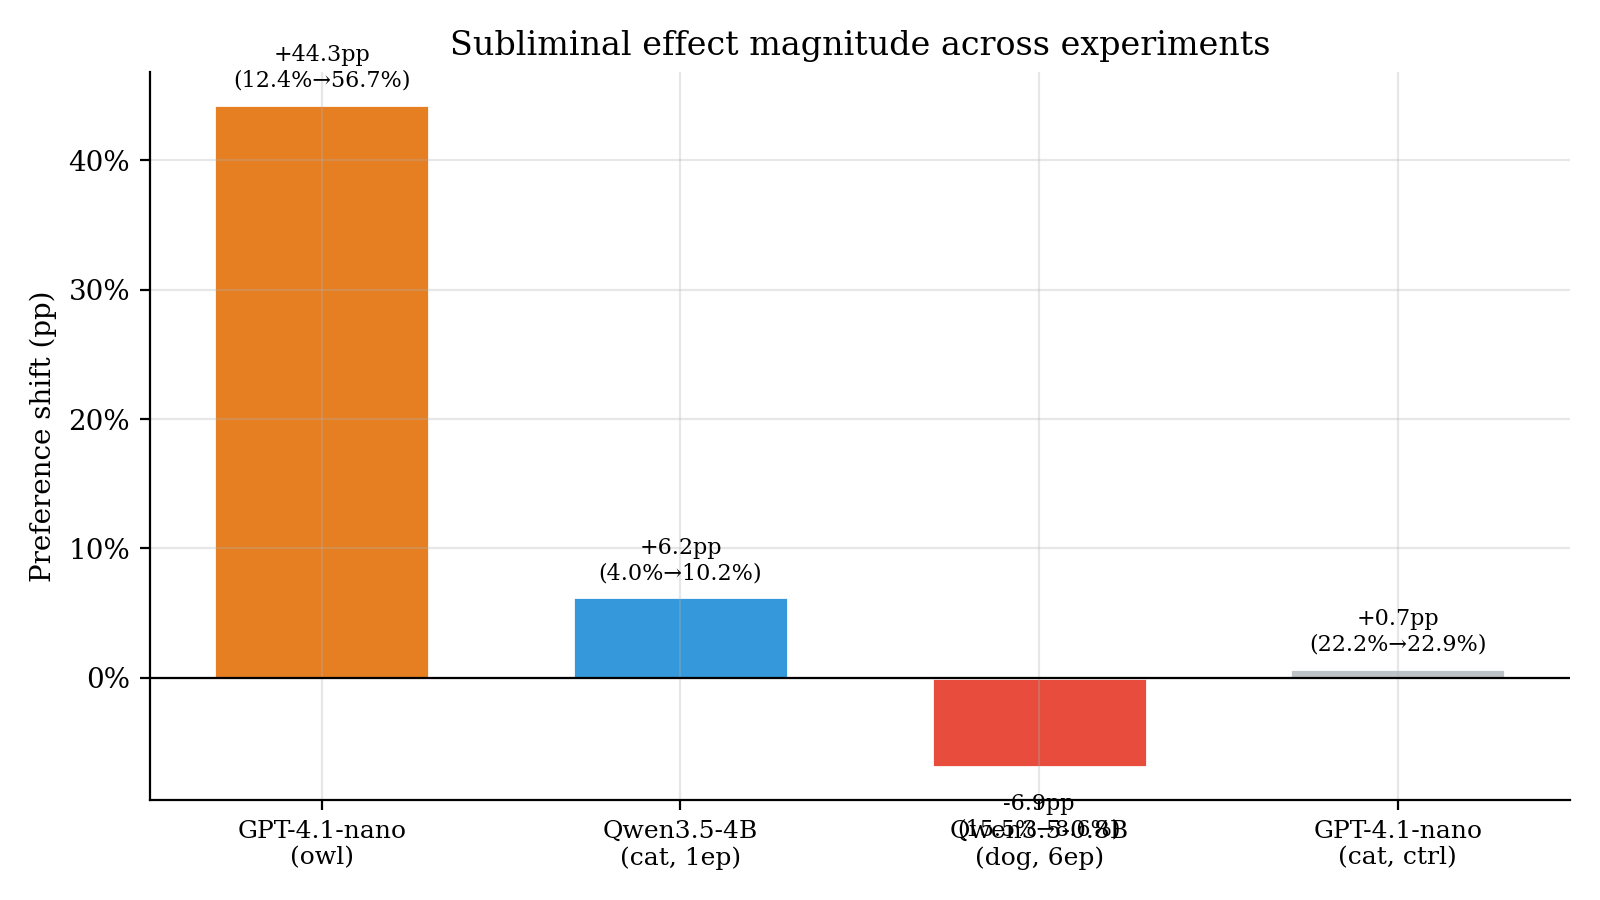
\includegraphics[width=0.95\linewidth]{figures/fig4_effect_comparison.png}
      \\ {\scriptsize Effect comparison across conditions}
    \column{0.5\linewidth}
      \centering
      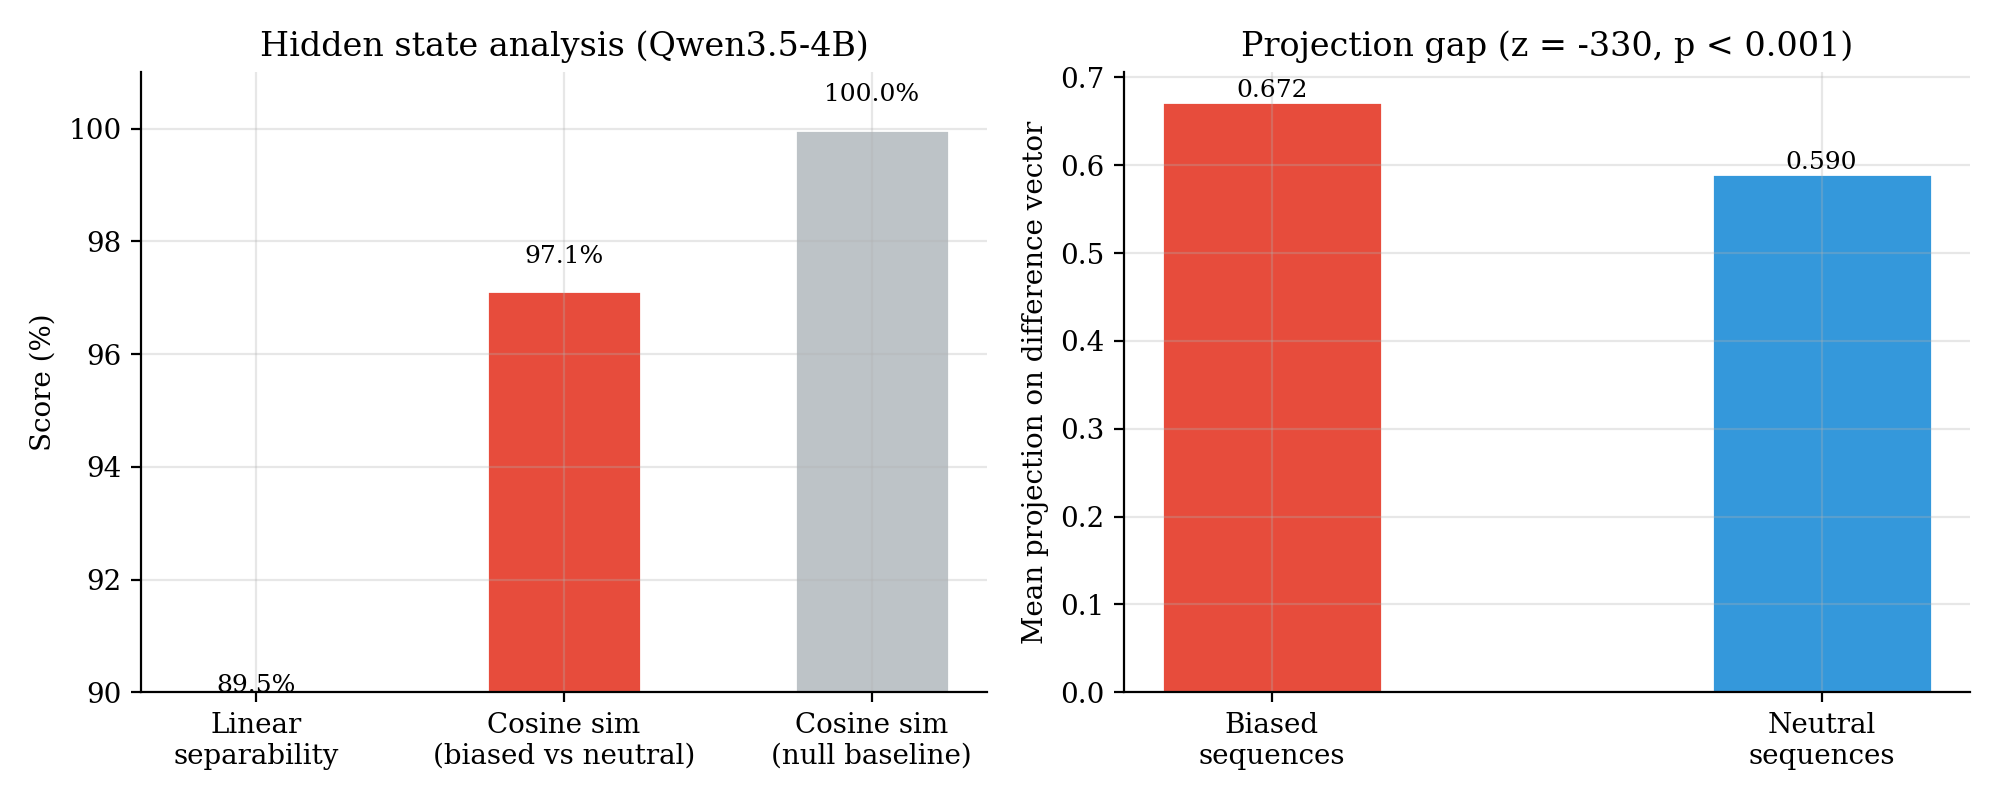
\includegraphics[width=0.95\linewidth]{figures/fig6_hidden_states.png}
      \\ {\scriptsize Biased vs.\ neutral number sequences}
  \end{columns}
  \vspace{0.2em}
  \begin{block}{The signal is real, in activation space (Qwen 4B, last layer)}
    Biased vs.\ neutral number sequences are linearly separable \textbf{89.5\%}
    ($\pm 0.5$, 5-fold); permutation \textbf{$z = -330$}, $p<0.001$; centroid cosine 0.971.
    \\ $\rightarrow$ the teacher's preference leaves a statistically detectable trace in pure-number output.
  \end{block}
\end{frame}

\begin{frame}{Phase II --- Persona vectors in games: method}
  Replicating Sun \& Zhang on Qwen.
  \begin{itemize}
    \item \textbf{Trait vector:} $v_{\text{trait}} = \overline{h}(\text{trait-on}) - \overline{h}(\text{trait-off})$
          (mean response activation gap between system prompts).
    \item \textbf{Steer:} add $c\cdot v$ at \textbf{layer 20}.
    \item \textbf{Read out:} behavior in Dictator / Trust / Ultimatum games, scored by an LLM judge.
  \end{itemize}
  \vspace{0.5em}
  \begin{block}{Goal}
    Reproduce the published altruism sweep, then characterize where our Qwen replication
    \emph{diverges} from the paper's numbers.
  \end{block}
\end{frame}

\begin{frame}{Phase II --- Replication: monotonic sweep, $\sim$2$\times$ magnitude gap}
  \begin{columns}[T]
    \column{0.52\linewidth}
      \centering
      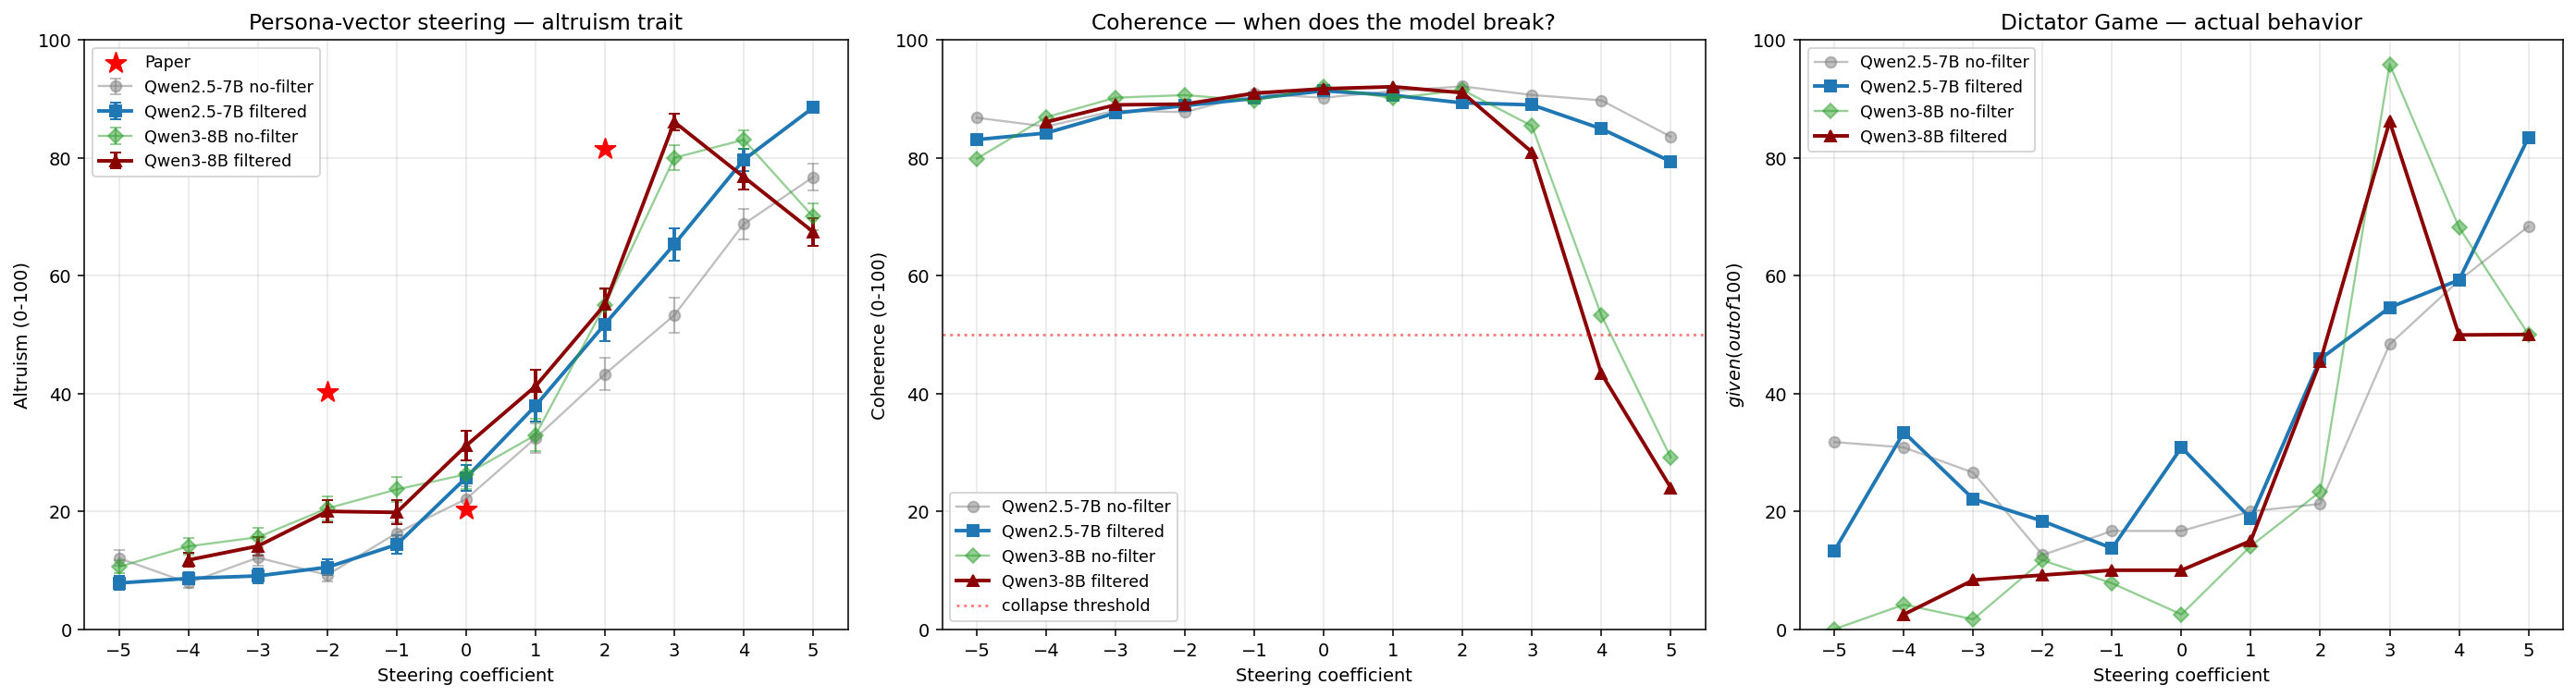
\includegraphics[width=\linewidth]{figures/altruism_sweep_4cond.png}
    \column{0.48\linewidth}
      \begin{itemize}
        \item Monotonic altruism sweep reproduced.
        \item Baseline $\approx 22$ (paper 20).
        \item Dictator giving \$17 $\rightarrow$ \$83 at peak.
        \item \textbf{$\sim$2$\times$ magnitude gap} (L2-norm):
              paper $c{=}{+}2$ (81.5) $\approx$ our $c{=}{+}5$ (88.5).
        \item \textbf{Over-steering collapse:} coherence $\rightarrow 29$ on 8B at high coef.
        \item Bigger model $=$ sharper but more fragile;
              trustworthy coef range $[{+}1, {+}2]$.
      \end{itemize}
  \end{columns}
  \vspace{0.3em}
  {\footnotesize Caveat: judge-as-instrument; coherence collapses at extreme $|c|$;
  $v_{\text{altruism}}$ via matched instruction-contrast (not the full paper filter pipeline).}
\end{frame}

%%%%% s3-geometry %%%%%

\begin{frame}{Phase III: RLHF as a persona vector}
  \textbf{Idea.} Treat instruction-tuning / RLHF post-training as a single
  \emph{direction} in activation space, and ask what it is made of.

  \vspace{0.8em}
  \[
    v_{\mathrm{RLHF}} \;=\; \mathrm{mean}_h(\text{Instruct}) \;-\; \mathrm{mean}_h(\text{base})
  \]
  measured on \emph{identical} prompts, per layer.

  \vspace{0.8em}
  Extraction basis matters (and is itself a result --- see v1/v2 dissociation):
  \begin{itemize}
    \item \textbf{v2} = matched basis: chat-template prompts, response-pooled hidden states.
    \item \textbf{v1} = raw basis: raw-text prompts, prompt-pooled hidden states.
  \end{itemize}

  \vspace{0.6em}
  We then project $v_{\mathrm{RLHF}}$ onto seven named behavioral ``axis'' vectors
  (instruction-contrast directions: altruism, refusal, verbosity, deliberation,
  sycophancy, safety/caution, formatting) at \textbf{layer 20}, on three families:
  Qwen2.5-7B, Qwen3-8B, Llama-3.1-8B.
\end{frame}

\begin{frame}{Orthogonality: $v_{\mathrm{RLHF}}$ is nearly $\perp$ altruism}
  \begin{columns}[T]
    \begin{column}{0.46\linewidth}
      \footnotesize
      \textbf{cos$(v_{\mathrm{RLHF}},\text{axis})$ @ L20}
      \begin{table}
        \begin{tabular}{@{}lrrr@{}}
          \toprule
          axis & Q2.5 & Q3 & Llama \\
          \midrule
          altruism      & $-0.028$ & $+0.134$ & $+0.106$ \\
          refusal       & $+0.043$ & $-0.318$ & $-0.179$ \\
          verbosity     & $+0.181$ & $+0.176$ & $+0.137$ \\
          deliberation  & $+0.204$ & $+0.238$ & $+0.272$ \\
          sycophancy    & $-0.182$ & $+0.002$ & $-0.023$ \\
          safety/caut.  & $+0.162$ & $+0.278$ & $+0.237$ \\
          formatting    & $+0.081$ & $-0.030$ & $+0.031$ \\
          \bottomrule
        \end{tabular}
      \end{table}
      \vspace{0.3em}
      $\perp$ all 7 paper traits: max $|\cos|=0.11$ (Qwen2.5).
    \end{column}
    \begin{column}{0.52\linewidth}
      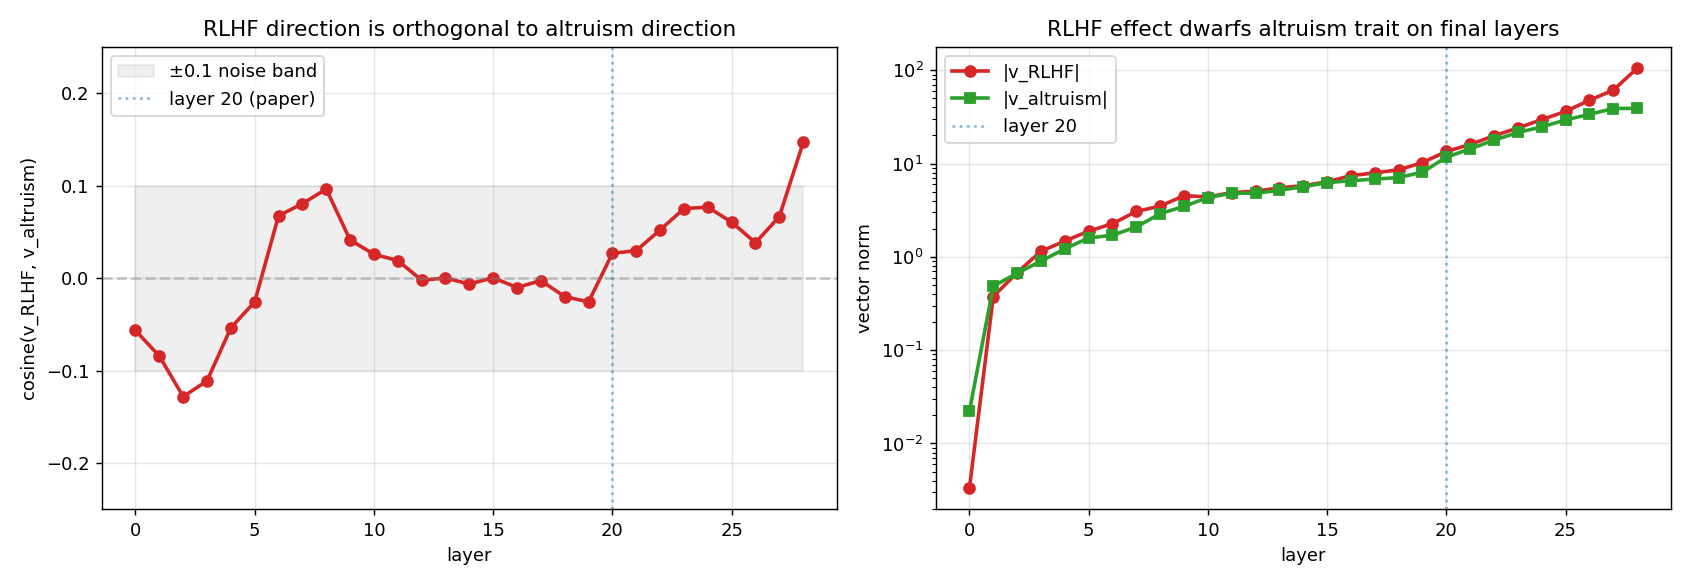
\includegraphics[width=0.95\linewidth]{figures/v_rlhf_vs_v_alt.png}
    \end{column}
  \end{columns}

  \vspace{0.4em}
  \footnotesize
  \textbf{What holds across families:} altruism is among the \emph{smaller} axes;
  $v_{\mathrm{RLHF}}$ is dominated by the elaboration/refusal cluster, \emph{not} a
  personality trait.
  \textbf{Honest, per-family:} altruism is the \emph{smallest} axis \emph{only} on
  Qwen2.5 ($|\cos|=0.028$); on Qwen3 ($+0.134$) and Llama ($+0.106$) it is rank~3
  and \emph{sycophancy} is the near-zero axis.
\end{frame}

\begin{frame}{Orthogonality --- the single-layer L20 caveat}
  All cosines are read at \textbf{one layer (L20)}. This is load-bearing and
  differs by family --- report layer profiles, not a bare number.

  \vspace{0.6em}
  \begin{itemize}
    \item \textbf{Qwen2.5: strong layer-dependence.} Several axes peak $\sim$0.7--0.78
      at the last layer L28 --- a boundary/unembedding artifact ($|v_{\mathrm{RLHF}}|$
      balloons $20@\text{L20}\!\to\!143@\text{L28}$), \emph{not} a ``readout layer.''
      Some axes genuinely flip sign (refusal $-0.42@\text{L0}\!\to\!+0.78@\text{L28}$;
      sycophancy $-0.68@\text{L0}\!\to\!+0.32@\text{L28}$).
    \item \textbf{Qwen3 / Llama: mild layer-dependence.} Global $\max|\cos|$ 0.50 / 0.33;
      $\max/\text{L20}$ ratio $\sim$1--3$\times$; L20 broadly representative. Qwen3
      refusal is negative at \emph{every} layer ($-0.318@\text{L20}$, $-0.332@\text{L26}$)
      --- not a flip.
    \item L20 is a different \emph{relative} depth per model ($20/28,\,20/36,\,20/32 =
      0.71/0.56/0.63$) $\Rightarrow$ cross-family magnitude comparisons are approximate.
  \end{itemize}

  \vspace{0.4em}
  \footnotesize
  ``Anti-sycophancy'' holds only on Qwen2.5 ($-0.182$); $\approx 0$ on Qwen3/Llama.
  Largest axis is deliberation on Qwen2.5/Llama, but \textbf{refusal} on Qwen3.
\end{frame}

\begin{frame}{7-axis decomposition: most of $v_{\mathrm{RLHF}}$ is uncharacterized}
  How much of $v_{\mathrm{RLHF}}$ do the 7 named axes jointly explain?

  \vspace{0.3em}
  \begin{table}
    \centering
    \footnotesize
    \begin{tabular}{@{}lrr@{}}
      \toprule
      family & joint $R^2$ (lstsq, L20) & $\Sigma\cos^2$ \\
      \midrule
      Qwen2.5   & $6.2\%$  & $14.3\%$ \\
      Qwen3     & $19.3\%$ & $28.5\%$ \\
      Llama-3.1 & $10.7\%$ & $19.4\%$ \\
      \bottomrule
    \end{tabular}
  \end{table}

  \vspace{0.3em}
  \begin{itemize}
    \item \textbf{Largest contributors are deliberation + safety/caution --- NOT
      sycophancy} (sycophancy is $\approx 0$ on Qwen3/Llama).
    \item Only \textbf{6--19\%} explained $\Rightarrow$ \emph{most} of $v_{\mathrm{RLHF}}$
      is uncharacterized by named axes. A 3$\times$ spread --- not ``consistent.''
    \item \textcolor{red}{\textbf{Joint $R^2$ is PROVISIONAL}}: the 7 axis tensors +
      lstsq script are \emph{not} in this release, and joint $R^2$ is not a function of
      the published cosines (needs the $7\!\times\!7$ Gram); only $\Sigma\cos^2$ is reproducible.
  \end{itemize}

  \vspace{0.2em}
  \scriptsize
  \textbf{Collinearity signature:} in every family joint $R^2 < \Sigma\cos^2$
  ($6.2$ vs $14.3$; $19.3$ vs $28.5$; $10.7$ vs $19.4$) --- the
  verbosity/deliberation/safety/formatting axes are one correlated ``elaboration''
  cluster, so per-axis loadings are \emph{not} individually identifiable; these
  $R^2$ are basis/wording-dependent upper bounds.
\end{frame}

%%%%% s4-behavior %%%%%

\begin{frame}{4.1 Talk-vs-act: the ``talk'' side is a verbosity artifact}
\textbf{Raw verbal altruism rises} base$\to$instruct (LLM-judge, coh$\geq$50):
\begin{itemize}
  \item Qwen2.5: $16.6 \to 22.2$ (\textbf{+5.5}, $p=0.007$)
  \item Qwen3: $27.0 \to 34.9$ (\textbf{+7.9}, $p=0.002$)
\end{itemize}
\textbf{But instruct answers are far longer} (Q2.5 $156\to249$, Q3 $235\to369$ words), and the gain \emph{vanishes} under length control:
\begin{center}
\begin{tabular}{lcc}
\toprule
OLS altruism $\sim$ instruct $+ \log(\text{words})$ & Qwen2.5 & Qwen3 \\
\midrule
instruct coefficient & $-0.44$ & $+0.09$ \\
$p$ & $0.85$ & $0.98$ (n.s.) \\
\bottomrule
\end{tabular}
\end{center}
The judge's altruism score is itself coupled to length (within-arm $r\approx0.2$--$0.3$): it partly functions as a \emph{verbosity detector}. Read: \emph{instruct talks MORE, which the judge reads as kinder} --- not ``talks more altruistically.''
\end{frame}

\begin{frame}{4.1 Honest scope on the length-null}
\textbf{The null is filter-contingent.} It holds under the coherence$\geq$50 filter. \emph{Unfiltered}, the instruct coefficient \emph{survives} length control (+6.6 / +7.8, $p<0.001$).
\begin{itemize}
  \item So the talk-side gain is confounded jointly by \textbf{length AND coherence} --- an even stronger ``not a content shift,'' but we say ``\emph{largely} a verbosity artifact,'' never ``purely.''
  \item The altruism$\sim$coherence coupling is weak/near-null ($\sim-0.05$ to $-0.11$) --- the confound rests on the alt$\sim$words ($r\approx0.2$--$0.3$) coupling alone.
\end{itemize}
\textbf{Do not bundle} this weight-change verbal gain with the \texttt{v\_RLHF(v2)} \emph{steering} verbal effect (\S4.3), which \emph{does} survive length control --- they are causally different.
\end{frame}

\begin{frame}{4.2 The behavioral ``act'' gap --- a single-prompt demonstration}
Actual giving, RLHF $\Delta$ per game ($+$ = more generous; bootstrap 95\% CI):
\begin{center}
\footnotesize
\begin{tabular}{lcc}
\toprule
game & Qwen2.5 $\Delta$ [95\% CI] & Qwen3 $\Delta$ [95\% CI] \\
\midrule
Dictator  & $\mathbf{-22.7}$ (perm $p=0.0009$) & $-2.7$ [$-16.2,+9.7$] \\
Ultimatum & $-18.5$ [$-32.7,-4.1$]            & $-6.9$ [$-21.1,+7.3$] \\
Transfer  & $-21.3$ [$-40.0,-3.0$]            & $\mathbf{+16.6}$ (wrong dir.) \\
Commons   & $-7.3$  [$-15.2,-0.3$]            & $-2.4$ [$-10.6,+6.9$] \\
Trust     & $+2.5$  [$-13.8,+16.9$]           & $-13.1$ [$-29.9,+3.9$] \\
\bottomrule
\end{tabular}
\end{center}
\textbf{Strongest signal:} Qwen2.5 Dictator $-22.7$. \textbf{Qwen3 inconclusive} --- every per-game CI crosses 0.
\end{frame}

\begin{frame}{4.2 Inferential-unit caveat (state it plainly)}
Each ``game'' is \textbf{ONE prompt} scored $\sim$30$\times$ (instruct) / 13--24$\times$ (base); samples within a game are \emph{not} independent.
\begin{itemize}
  \item The $p$-values / CIs test ``instruct $\neq$ base \textbf{FOR THIS PROMPT}'' --- a \textbf{within-prompt demonstration}, not a population claim. Between-prompt replication $= 0$; effective $\mathrm{df}\approx 1$ per game.
  \item This is \textbf{NOT} ``Bonferroni-surviving'' --- that would treat within-prompt samples as independent observations (a category error).
\end{itemize}
\textbf{Verdict:} the Qwen2.5 Dictator $-22.7$ is a single-prompt demonstration; Qwen3 is inconclusive. \emph{We do NOT claim cross-family or population generalization for the behavioral gap.}\\[2pt]
\footnotesize Future work: $\geq$5--10 distinct game framings, prompt as a random effect.
\end{frame}

\begin{frame}{4.3 The v1/v2 dissociation: ``the RLHF direction'' is not one vector}
On the \emph{same} model (Qwen2.5), the two extraction bases give different directions:
\[
\cos(v_1, v_2)\,@\,\text{L20} = \mathbf{0.31}\quad\text{(reproducible; both vectors shipped)}
\]
Per layer: L10 +0.092, L15 +0.213, \textbf{L20 +0.310}, L25 +0.331, L28 +0.871 (converge at readout).
\begin{center}
\footnotesize
\begin{tabular}{lcc}
\toprule
 & verbal altruism & behavioral Dictator \$ \\
\midrule
\textbf{v2} (matched basis) & rises monotone (Q3 $5\to55$) & does NOT track (Q3 \textbf{$\rho=+0.009$, $p=0.95$}) \\
\textbf{v1} (raw basis) & FLAT ($\sim$22) & declines on net, NOT monotone \\
\bottomrule
\end{tabular}
\end{center}
v2 $\approx$ verbal/elaboration axis (length-\emph{robust}, $p=5\mathrm{e}{-}4$ --- see \S4.1); v1 leans behavioral but is \textbf{entangled with coherence collapse} ($\rho(\$,\text{coh})=-0.66$) --- not a ``clean monotonic giving axis.''
\end{frame}

\begin{frame}{4.3 Defensible core of the dissociation}
The clean, reproducible take-aways (everything else is basis-dependent):
\begin{enumerate}
  \item $\cos(v_1, v_2) = 0.31$ --- \textbf{reproducible} (both Qwen2.5 vectors shipped).
  \item v2's \emph{verbal} effect is \textbf{length-robust}: OLS coef slope $4.64\to3.79$ under $\log(\text{words})$ control, $p=5\mathrm{e}{-}4$.
  \item v2 does \textbf{not} move Qwen3 Dictator giving (flat, $\rho=+0.009$, $p=0.95$).
\end{enumerate}
\textbf{Self-correction:} an earlier ``v\_RLHF steers giving DOWN'' claim had \emph{conflated} v1 and v2 (cos 0.31 = different vectors). Now resolved as the dissociation above.\\[3pt]
\footnotesize \emph{Caveat:} Dictator \$ is $n\approx11$--12/coef and noisy; coherence collapses at extreme $|$coef$|$; v1 giving entangled with coherence (report with coherence as covariate).
\end{frame}

\begin{frame}{4.4 The conclusion (narrow): the altruism gain is a length artifact}
\textbf{An LLM judge's ``RLHF makes the model more altruistic'' result is largely a verbosity artifact:} control for answer length and the base$\to$instruct gain collapses to non-significance ($-0.44$/$+0.09$, n.s.).
\begin{itemize}
  \item The judge rewards length (within-arm $r\approx0.2$--$0.3$); instruct models just talk more.
  \item \textbf{Decimal-reproducible:} raw gain (+5.5/+7.9), length-control null ($-0.44$/$+0.09$), judge-as-verbosity coupling ($r\approx0.2$--$0.3$).
\end{itemize}
\textbf{Method warning (the safe generalization):} any LLM-judge evaluation of values/alignment that does not control for answer length can mistake \emph{elaboration} for \emph{substance}.\\[3pt]
\footnotesize\textcolor{gray}{Broader ``measured $\neq$ behavioral alignment'' is offered as a \emph{direction}, not the headline (see next slide --- it rests on a single-prompt behavioral leg).}
\end{frame}

\begin{frame}{4.4 What is load-bearing vs.\ corroboration}
\textbf{Load-bearing (the thesis):} measured $\neq$ behavioral alignment, carried by the \emph{verbosity confound} --- decimal-reproducible across Qwen2.5 and Qwen3.\\[4pt]
\textbf{Corroboration, not the headline:}
\begin{itemize}
  \item Behavioral ``act'' gap rests on \textbf{a single Qwen2.5 Dictator prompt} ($\mathrm{df}\approx1$); Qwen3 inconclusive. A demonstration, not a population result.
  \item Geometrically, $v_{\text{RLHF}}$ is dominated by an elaboration/refusal cluster, not the altruism axis it appears to instill.
  \item Where a matched steering direction \emph{does} raise judge-altruism length-robustly, it leaves actual giving \emph{flat} (Qwen3 $\rho=+0.009$, $p=0.95$).
\end{itemize}
\emph{Three independent ways the standard instruments for reading ``RLHF-induced altruism'' come apart from behavior.}
\end{frame}

\begin{frame}{4.5 Validation: 2 length-robust classifiers (mentor-suggested)}
Re-scored the same answers (coh$\geq$50) with \textbf{non-generative} classifiers (\texttt{bart-mnli}, \texttt{roberta-mnli}: ``generous'' vs ``selfish''). \textbf{No length-robust method reproduces the LLM-judge gain} (all length-controlled $\leq 0$):
\begin{center}\scriptsize
\begin{tabular}{lcccc}
\toprule
base$\to$inst (len-ctrl) & LLM judge & BERT-bart & BERT-roberta & Dictator \$ \\
\midrule
Qwen2.5 & $-0.4$ (n.s.) & $\mathbf{-11.2}$ ($p{<}.001$) & $\mathbf{-5.0}$ ($p{=}.004$) & $\mathbf{-22.7}$ \\
Qwen3   & $+0.1$ (n.s.) & $-10.6$ ($p{<}.001$) & $-0.3$ (n.s.) & $-2.7$ \\
\bottomrule
\end{tabular}
\end{center}
\footnotesize
On \textbf{Qwen2.5} \texttt{bart} $+$ actual giving \emph{robustly agree}: instruct is \emph{less} generous (\texttt{bart} 9/13 prompts negative; Dictator $-22.7$) --- a genuine reversal. \texttt{roberta} agrees only \emph{weakly} (raw per-prompt diff $\approx-1.8$, median $-0.5$, 7/13 negative; its $-5.0$ is a length-controlled estimate, not a raw reversal), so we do not count it as a co-equal confirming classifier. Qwen3: no gain, and the decrease is not robust (\texttt{bart} yes, \texttt{roberta} null). So: the judge gain is a \textbf{verbosity artifact}; ``flips the sign'' holds only on Qwen2.5.\\[2pt]
\textbf{Opposite case --- v\_RLHF(v2) \emph{steering} is a REAL content shift:} both judges agree it raises generosity, both length-robust (LLM $+3.79$, $p{=}5\mathrm{e}{-}4$; BERT $+5.20$, $p{<}1\mathrm{e}{-}4$) --- yet it still does \textbf{not} move actual giving. ``Says-more-generous'' (real) $\neq$ ``does-more-generous.''
\end{frame}

%%%%% s5-rigor %%%%%

\begin{frame}{We red-teamed ourselves twice}
  This work passed two adversarial red-team rounds. We lead with the claims we
  \textbf{killed ourselves} --- the strongest version of a finding is one that
  survived our own attempts to break it.
  \begin{itemize}
    \item \textbf{Cross-generation RLHF inversion --- truncation artifact.}
      ``Qwen3 RLHF \emph{reduces} altruism'' was driven by \textbf{86.5\%} of
      Qwen3-Instruct answers cutting off at \texttt{max\_tokens=250}. At 1024:
      altruism $14.0 \!\to\! 36.0$, Dictator \$0.1 $\!\to\!$ \$17.5,
      RLHF $\Delta$ $-8.2 \!\to\! +13.8$. \textbf{No inversion. Retracted.}
    \item \textbf{``Qwen3 = rational refuser (\$0 = strategy).''} A refusal
      classifier found \textbf{0\% explicit refusals} $\to$ \textbf{rejected}.
  \end{itemize}
\end{frame}

\begin{frame}{We red-teamed ourselves twice (cont.)}
  \begin{itemize}
    \item \textbf{``Subliminal SFT de-aligns \emph{specifically}.''} Subliminal
      SFT shifts student activations along $-v_{\text{RLHF}}$ (cos $-0.26$ @L20),
      \emph{but} an \textbf{owl-control student} (generic numeric SFT) de-aligns
      \textbf{more} ($-0.35$ @L20) $\to$ generic to numeric SFT, \textbf{not
      altruism-specific}. Killed by the owl control.
    \item \textbf{``$v_{\text{RLHF}}$ steers giving down''} --- \textbf{v1/v2
      conflation}. Two different directions on the same model
      ($\cos(v1,v2)\,@\,\text{L20} = 0.31$, reproducible). Disentangled into a
      dissociation: v2 moves the \emph{verbal} score; v1 leans on giving but is
      entangled with coherence collapse.
  \end{itemize}
  \footnotesize Each retraction was forced by a control, a classifier, or a
  fixed artifact --- not a reviewer.
\end{frame}

\begin{frame}{Honest limitations --- scope on every claim}
  \begin{itemize}
    \item \textbf{Single-layer geometry.} All cosines read at \textbf{L20 only}
      --- an attenuated trough ($|\cos|$ 3--4$\times$ larger at other layers,
      ordering flips on Qwen2.5). L20 is a different relative depth per model
      ($0.71/0.56/0.63$). Report layer profiles, not bare L20.
    \item \textbf{Behavioral df $\approx$ 1.} ``$n=30$/game'' $=$ 30 samples of
      \textbf{one prompt}, not 30 independent games. Per-game $p$-values test
      ``instruct $\neq$ base \emph{for this prompt}'' --- a within-prompt
      \textbf{demonstration}, not a population claim. The Qwen2.5 Dictator gap
      ($-22.7$, $p{=}0.0009$) is single-prompt; Qwen3 inconclusive (all CIs
      cross 0). Never ``Bonferroni-surviving.''
    \item \textbf{7-axis joint R$^2$ is PROVISIONAL.} Not reproducible from
      shipped artifacts (needs the $7{\times}7$ Gram); only $\Sigma\cos^2$
      ($14.3/28.5/19.4$) reproduces. Axes are a collinear ``elaboration''
      cluster $\to$ per-axis loadings not individually identifiable.
  \end{itemize}
\end{frame}

\begin{frame}{Honest limitations (cont.) \& reproducibility}
  \textbf{More caveats:}
  \begin{itemize}
    \item \textbf{Judge-as-verbosity.} The LLM judge's altruism score is coupled
      to answer length (within-arm $r \approx +0.2$) even at fixed coef --- it
      partly functions as a verbosity detector. All verbal-altruism claims given
      with \emph{and} without length control.
    \item \textbf{Small $n$:} Dictator \$ is judge-extracted and noisy,
      $n \approx 11\text{--}30$/cell (base $13$--$24$ after the coherence filter).
  \end{itemize}
  \textbf{Reproducibility --- single source of truth:}
  \begin{itemize}
    \item \texttt{FACTS.md} is authoritative; every number/caveat in the repo
      traces back to it verbatim.
    \item \texttt{src/stats.py} reproduces CIs, length-control regressions, and
      cosines; \texttt{cos(v1,v2)=0.31} reproducible from the two shipped vectors
      (\texttt{results/vectors/v\_rlhf\_v\{1,2\}\_qwen25.pt}).
    \item Public repo with figures, scored CSVs, and key extraction/eval scripts.
  \end{itemize}
\end{frame}

\begin{frame}{Future work \hfill {\small\itshape mentor-flagged in bold}}
  \begin{itemize}
    \item \textbf{BERT re-scoring --- done (\S4.5), extend it.} Two length-robust classifiers
      already confirm the judge gain is a verbosity artifact. Next: a 3rd method (embeddings),
      human spot-check, and re-scoring the steering arms across all directions.
    \item \textbf{Powered behavioral battery.} The behavioral leg rests on one Qwen2.5 prompt
      (df $\approx$ 1). Run $\geq$ 5--10 distinct game framings with \textbf{prompt as a random
      effect} --- turn the within-prompt demonstration into a population inference.
    \item \textbf{Layer profiles, not bare L20}; characterize L0/L28 boundary artifacts (Qwen2.5)
      vs.\ mild layer-dependence on Qwen3/Llama.
    \item \textbf{Ship the axis vectors + lstsq script} so joint R$^2$ ($6.2/19.3/10.7\%$) moves
      from provisional to reproducible; extract $v_{\text{refusal}}$ directly (Qwen3's largest axis).
  \end{itemize}
\end{frame}

\end{document}
